\section{Entwurfsentscheidungen}
\label{sec:fachkonzept-entwurf}

\autorbeginn{Fredrik}

\subsection{Einleitung}
Zur Erstellung eines Unternehmensplanspiels bedarf es - wie in jedem Prozess der Software-Erstellung - nach einer anfänglichen Analyse der benötigten Funktionalität, deren Ergebnisse in \ref{sec:fachkonzept-usecase} anhand eines Use Case Diagramms verkürzt dargestellt wurden, Entscheidungen zum grundlegenden Entwurf der Software. Diese Phase grenzt sich klar ab von den Entscheidungen zur Implementierung des Projekts, die in \ref{sec:fachkonzept-implementierung} erläutert werden, da sie sich auf einem höheren Abstraktionsniveau bewegt. Es geht hierbei nicht darum, die Lösung auf eine bestimmte Umsetzung hin zu optimieren, sondern die erkannten Anforderungen weitestgehend zu ermöglichen. Diese Entscheidungen sollen strukturiert werden mit Hilfe der Notation des UML Klassendiagramms.

Konkret bedeutet der höhere Abstraktionsgrad, dass Eigenheiten wie die System-Architektur (z.B. Client-Server-Architektur), die Persistierung von Daten oder die Benutzeroberfläche an dieser Stelle weder behandelt noch berücksichtigt werden sollen. Im Vordergrund stehen stattdessen die SpielWelt und alle Elemente, die den Ablauf des Spiels ermöglichen. Um eine gewisse Übersichtlichkeit zu gewährleisten, wurde auf die Aufführung von \textit{get()}- und \textit{set()}-Methoden verzichtet, solange diese als trivial einzustufen sind. Ebenso gilt für alle Assoziationen die Annahme, dass diese mit der Kardinalität 1:1 zu verstehen sind, außer es sind abweichende Kardinalitäten eingetragen.

Aufgrund der Größe des Klassendiagramms ist dies erst in \vref{sec:anhang-klassendiagramm} vollständig dargestellt. Im Folgenden sollen einige Bereiche aus diesem Modell getrennt voneinander betrachtet werden. Nach einer Vorstellung des Modellkerns werden zunächst die sogenannten Typen, die Beschreibungen von konkreten Gegenständen der Spielwelt wie z.B. den Raumschifftypen darstellen, betrachtet. Daran schließt sich eine Erläuterung der Märkte an, gefolgt von einer Betrachtung der Abteilungen. Zuletzt werden die zur Erfassung der Vorgänge in der Spielwelt und deren Speicherung dienenden Transaktions-Klassen erörtert.

\subsection{Die Kernelemente}
\begin{figure}[ht]
     \centering
     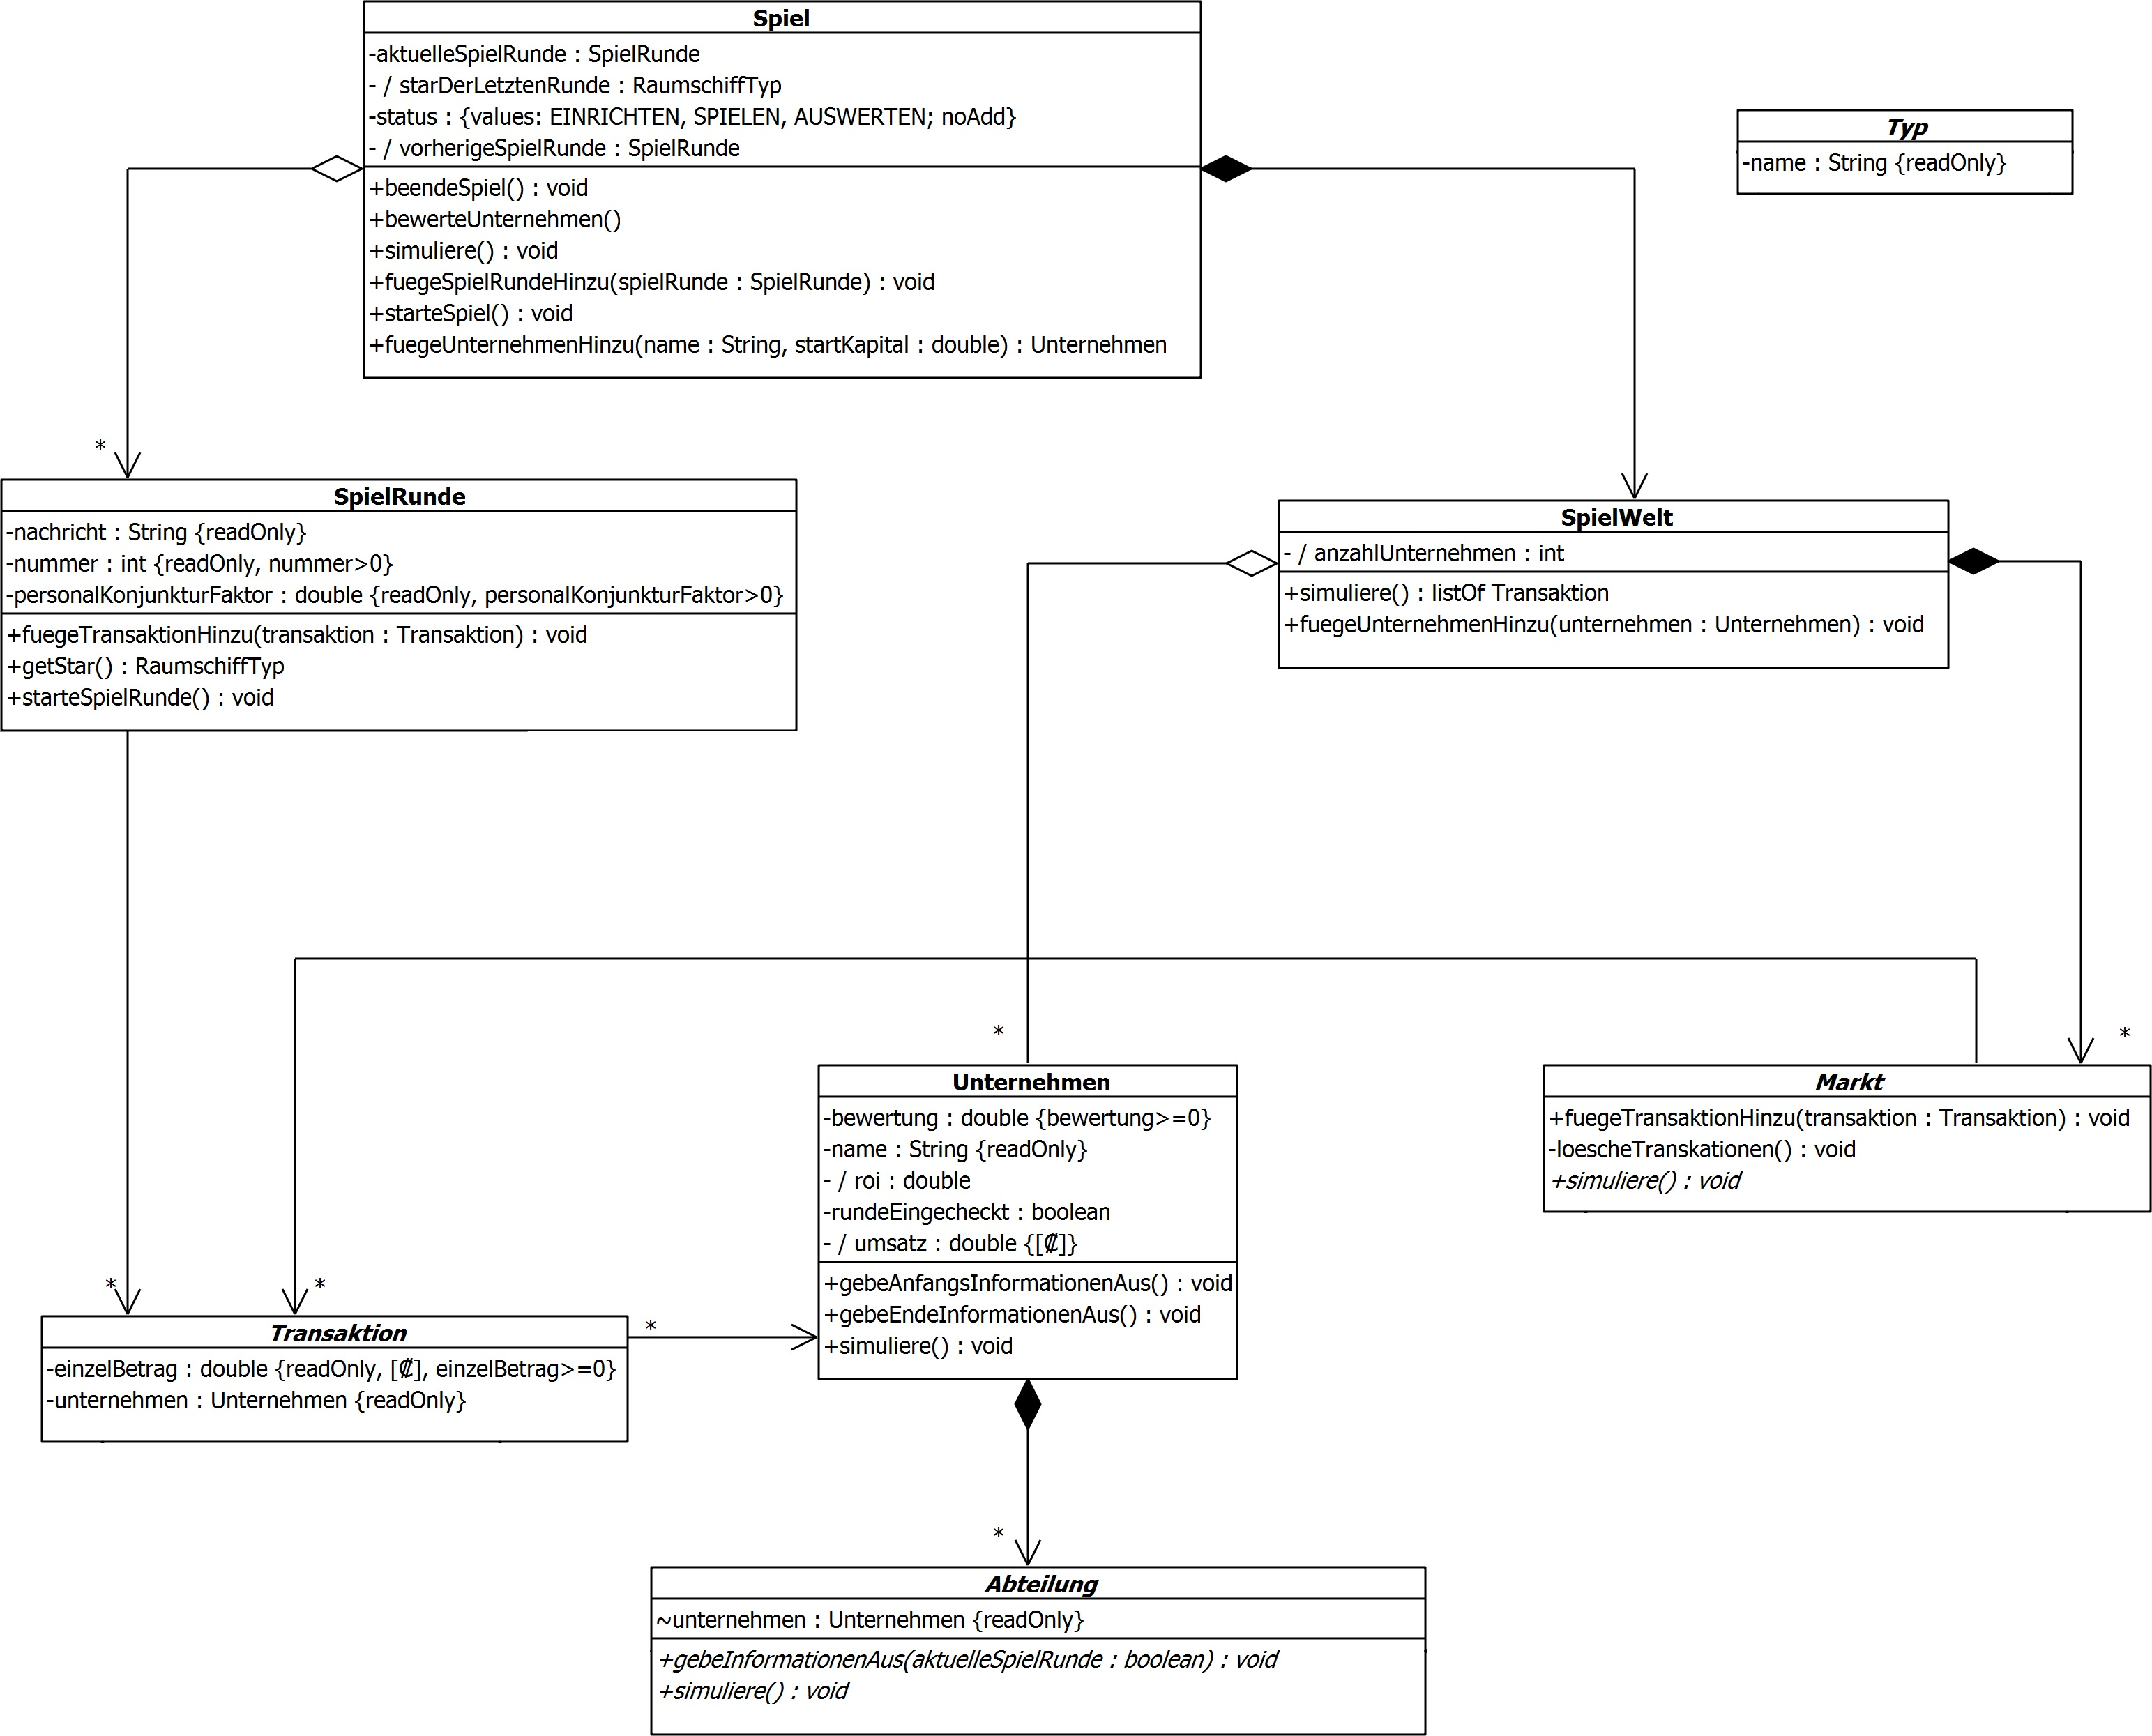
\includegraphics[width=\textwidth]{30_Fachkonzept/20_Entwurf/kern}
     \caption{Klassendiagramm - Kernelemente}
     \label{img:fachkonzept-entwurf-kern}
\end{figure}

In \ref{img:fachkonzept-entwurf-kern} sind die Kernelemente des Entwurfsmodells zu sehen. Hieran lässt sich gut erkennen, dass \textit{Spiel} die zentrale Klasse darstellt. Sie steht in Verbindung mit der \textit{SpielWelt}, die für die eigentliche Simulation der wirtschaftlichen Vorgänge verantwortlich ist und daher auch mit den \textit{Märkten} und \textit{Unternehmen} verbunden ist. Ein Unternehmen besteht dabei aus mehreren \textit{Abteilungen}. Unabhängig von der Ebene der SpielWelt muss eine Speicherung der Vorgänge über das gesamte Spiel hinweg erfolgen, realisert durch die Klasse \textit{SpielRunde}. Diese dient zu Beginn des Spiels zur Aufnahme der Daten für den Spielverlauf wie Nachfrage-Entwicklung und Benachrichtigungen für den Spieler; im Verlauf des Spiels nimmt sie die Daten der abgeschlossenen Periode in sich auf um diese für die abschließende Bewertung verfügbar zu machen. Möglich wird die Speicherung aller erdenklichen Vorgänge durch die Klasse \textit{Transaktion}, die eine Handlung eines Spielers repräsentiert. Bisher ohne Verbindung zu den anderen Klassen steht \textit{Typ}, welches die Oberklasse für alle speziellen Typen (\textit{BauteilTyp} etc.) darstellt. Die Verbindungen ergeben sich erst bei näherer Betrachtung der einzelnen Sektionen.

An dieser Stelle soll hervorgehoben werden, dass die Ablauflogik des Spiels von der Methode \textit{simuliere()} in der Klasse \textit{Spiel} ausgeht, die einerseits die Simulation der SpielWelt vorantreibt, in der dann Absatzmengen und Bauteilpreise berechnet werden, und andererseits alle alten Transaktionen abspeichert um eine neue SpielRunde einzuleiten, wobei sich Auswirkungen auf die SpielWelt ergeben.

\subsection{Die Typen}
\begin{figure}[ht]
     \centering
     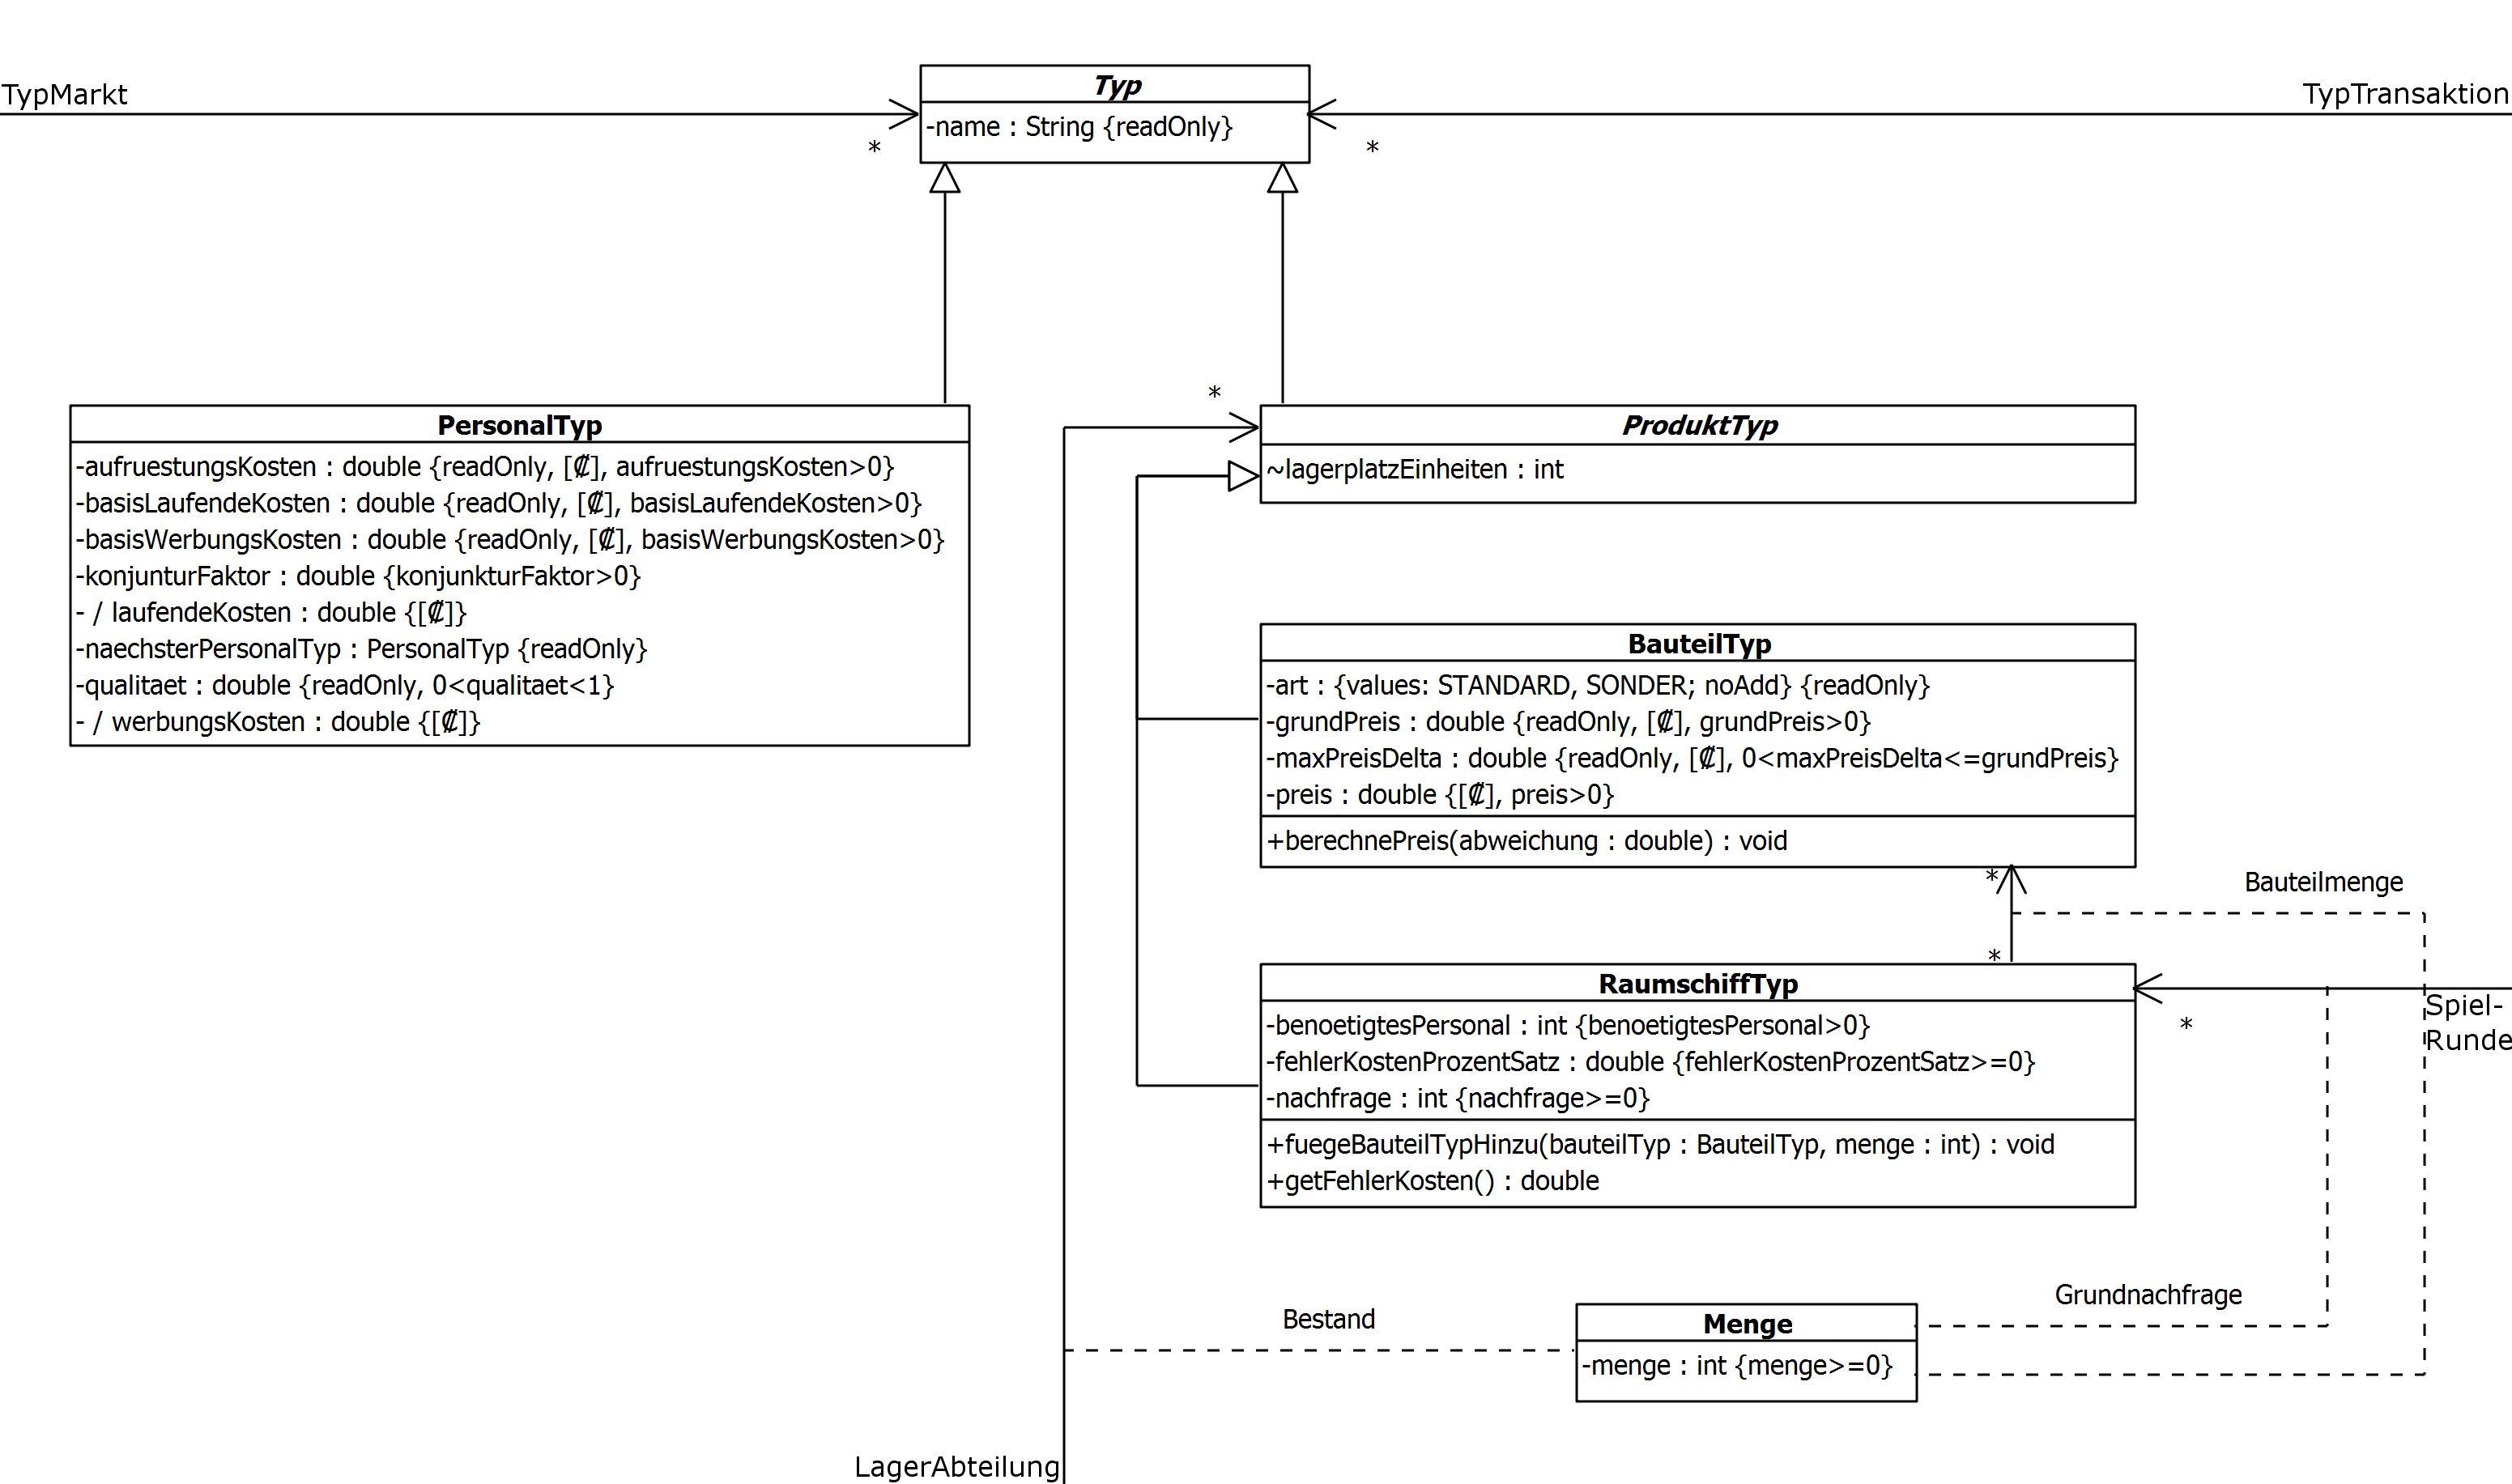
\includegraphics[width=\textwidth]{30_Fachkonzept/20_Entwurf/typ}
     \caption{Klassendiagramm - Typen}
     \label{img:fachkonzept-entwurf-typ}
\end{figure}

Der Begriff \textit{Typen} bezeichnet, wie oben bereits erwähnt, eine Beschreibung einer Gruppe von Gegenständen der Spielwelt. Es wurde bewusst auf eine Erzeugung jedes einzelnen Objekts in der Spielwelt verzichtet, um die Anzahl der benötigten Objekte nicht Überhand nehmen zu lassen. Obgleich diese Entscheidung vielleicht wie ein Vorgriff auf den Abstraktionsgrad der Implementierung wirkt, wurde hierdurch versucht, die Schere zwischen dem Modell der Entwurfs- und dem der Implementierungsphase möglichst gering zu halten, vor allem da sich die gewählte Möglichkeit nicht negativ auf die Funktionalität auswirkt. Die Gemeinsamkeit, die allen Typen innewohnt, ist der Name, der daher in einer Oberklasse definiert wurde.

Erkannt und umgesetzt wurde dabei die folgenden Typen, die ihrerseits von der Klassen \textit{Typ} erben:
\begin{seList}
\item \textbf{PersonalTyp:} Die für das Spiel notwendigen Personaltypen zeichnen sich einerseits durch ihren Qualitätsgrad, der die entstehenden Fehlerkosten beeinflusst, und andererseits durch die mit ihnen verbundenen Kosten aus. Hierzu gehören die Werbungskosten, die laufenden Kosten sowie die Aufrüstungskosten, wobei die ersten zwei abhängig von der Konjunktur auf dem Personalmarkt variieren können. Zusätzlich wird derjenige Personaltyp, auf den eine Aufrüstung erfolgen kann, gespeichert.
\item \textbf{BauteilTyp:} In der Spielwelt des Planspiels können Bauteiltypen entweder die Rolle von Standard- oder Sonderbauteilen annehmen, wobei erstere für jeden Raumschifftyp benötigt werden. Da dies in der Berechnung der neuen Bauteilpreise berücksichtigt werden muss, wird diese Eigenschaft abgespeichert. Zudem kann der Preis eines Bauteiltypen variieren, sodass neben dem Grundpreis auch die maximale Abweichung von diesem und der aktuelle Preis gespeichert werden müssen.
\item \textbf{RaumschiffTyp:} Diese setzen sich aus verschiedenen Bauteilen zusammen, wobei Bauteile mehrfach benötigt werden können. Daher wurde die assoziative Klasse \textit{Menge} eingeführt, die an anderen Stellen ebenfalls Verwendung findet. Zudem benötigt ein Raumschifftyp eine gewissen Menge Personal in einer Runde zur Herstellung, und verursacht bei fehlerhaften Herstellung einen gewissen Prozentsatz an Fehlerkosten, gemessen an dem aktuellen Preis der Bauteile, aus denen er sich zusammensetzt.
\end{seList}

Da sowohl Raumschifftypen als auch Bauteiltypen im Unternehmen gelagert werden können und für die Berechnung der hierdurch anfallenden Kosten der hierfür benötigte Platz Beachtung findet, erben beide von der abstrakten Klasse \textit{ProduktTyp}. Ein Raumschiff verbraucht dabei so viel Platz wie die Summe seiner Bauteile.

\subsection{Die Märkte}
\begin{figure}[ht]
     \centering
     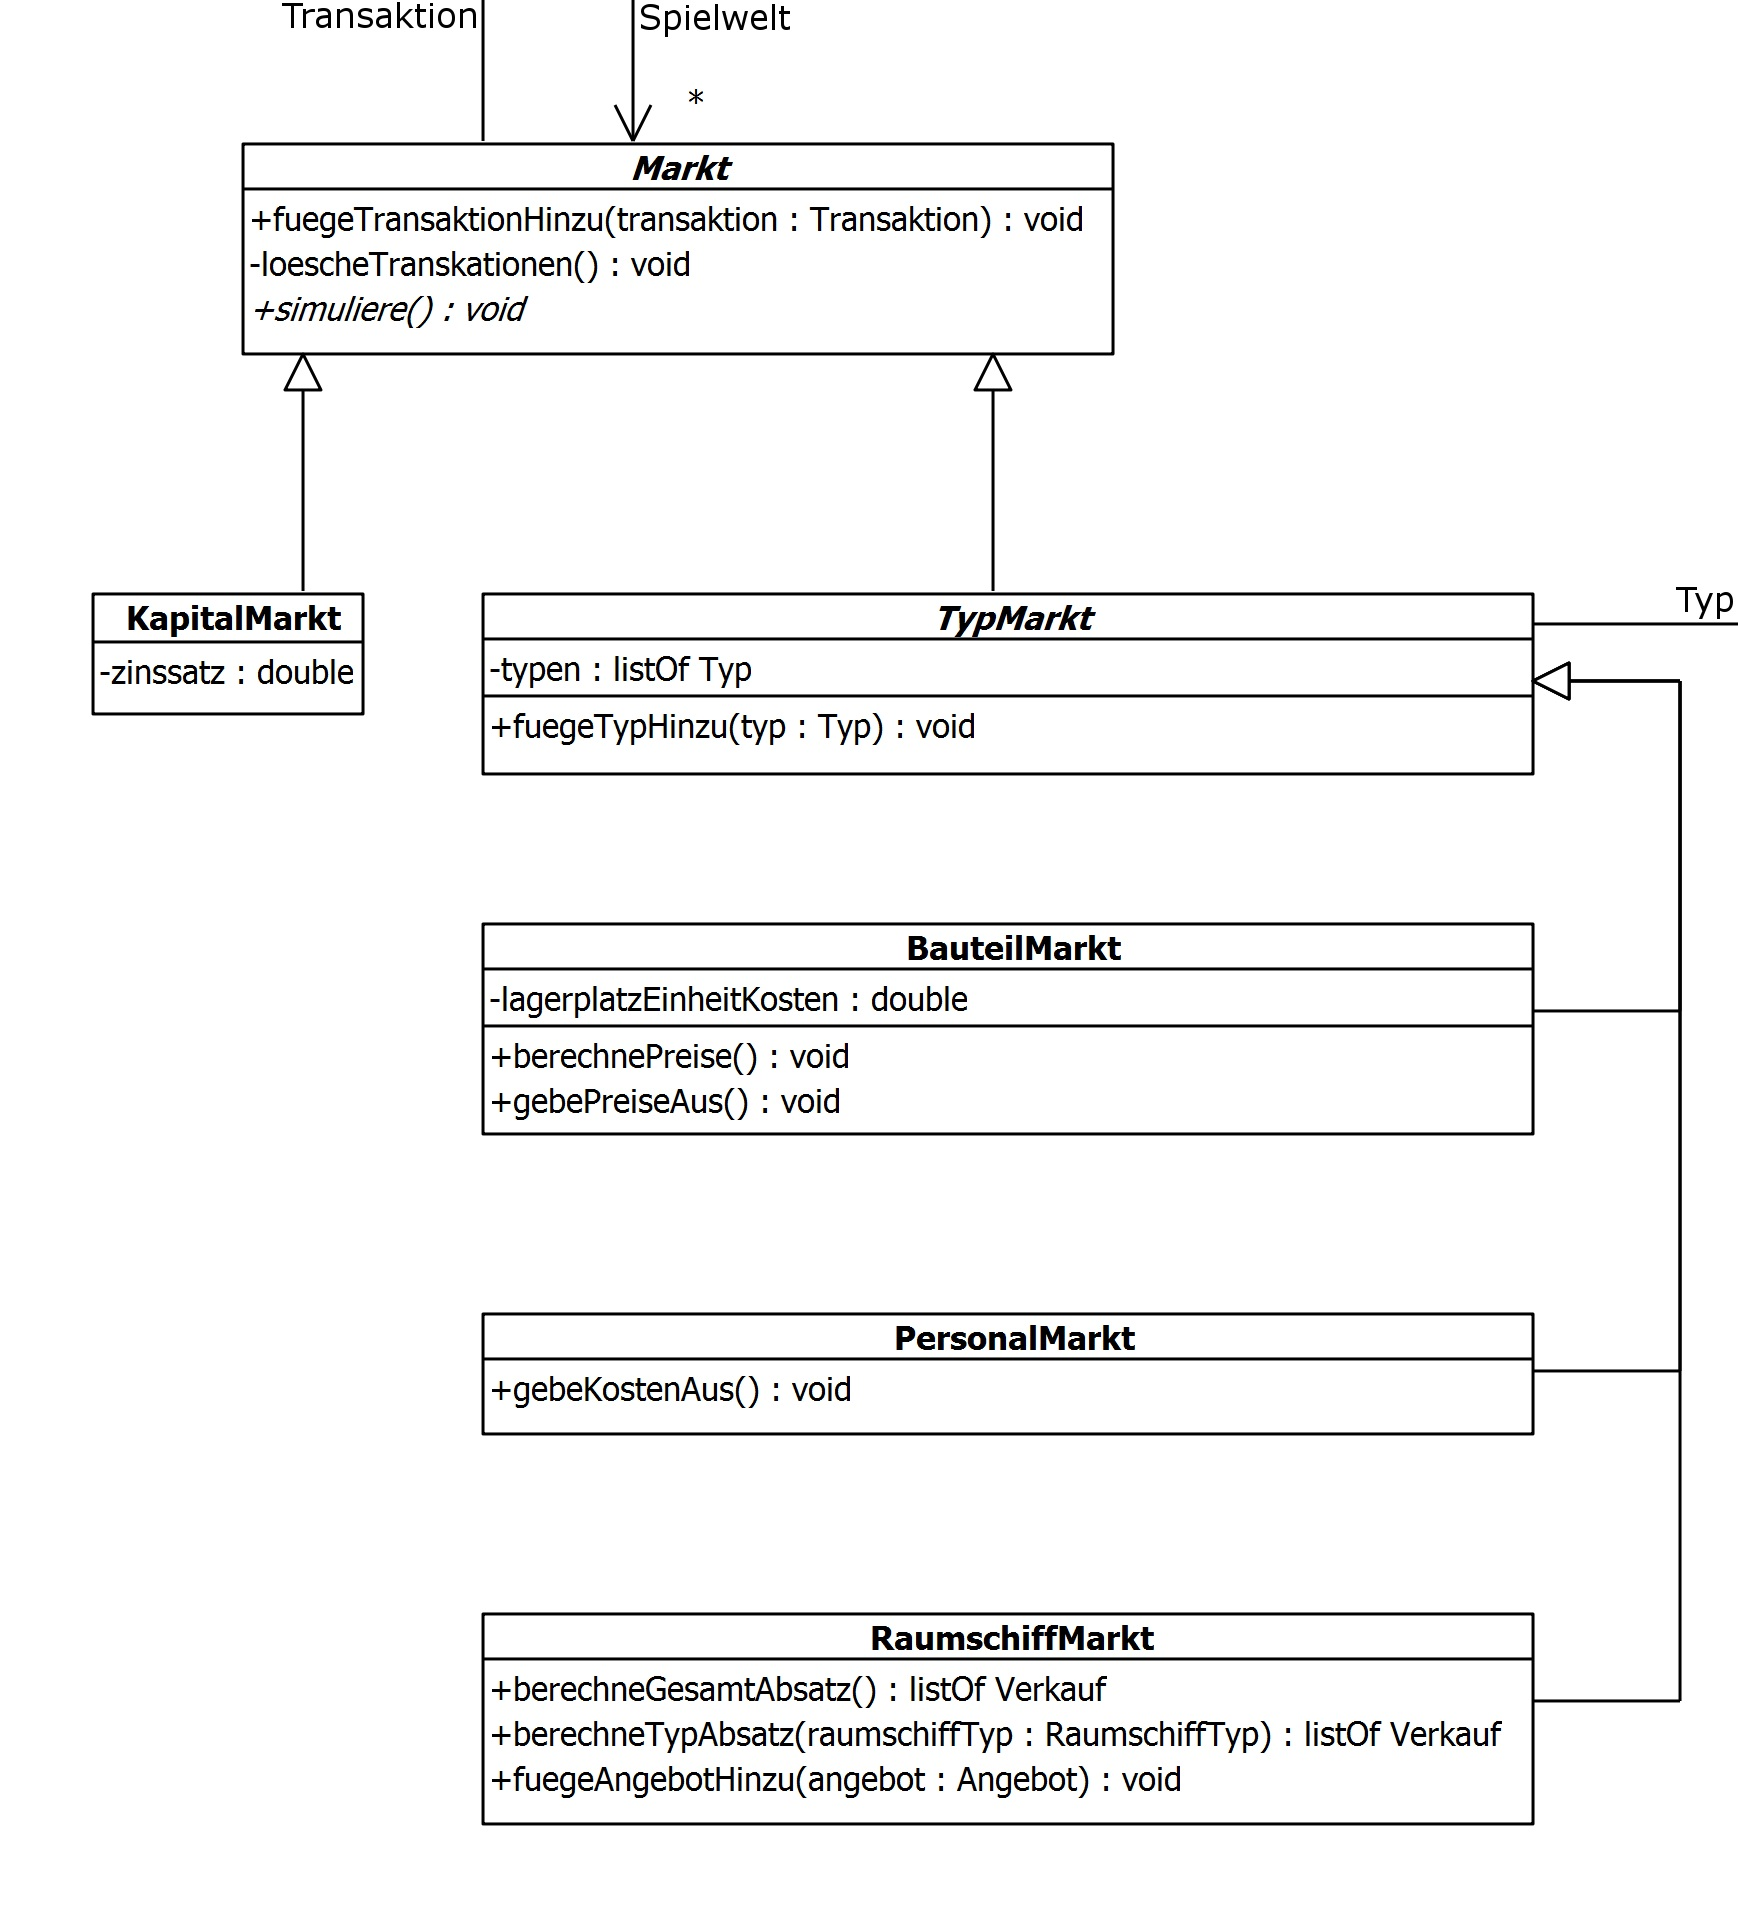
\includegraphics[width=0.7\textwidth]{30_Fachkonzept/20_Entwurf/markt}
     \caption{Klassendiagramm - Märkte}
     \label{img:fachkonzept-entwurf-markt}
\end{figure}

Im Planspiel gibt es verschiedene Märkte, die alle die zu ihnen gehörenden aktuellen Transaktionen verwalten. Betrachtet man diese näher, lässt sich feststellen, dass die meisten ebenfalls mit einer Art von \textit{Typ} in Verbindung stehen, wobei sie diese Typen auch verwalten sollen. Aus dieser Überlegung heraus ergibt sich die abstrakte Klassen \textit{TypMarkt}. Es folgt nun eine Erläuterung der einzelnen Märkte im Detail:

\begin{seList}
\item \textbf{Raumschiffmarkt:} Dieser Markt ist vermutlich derjenige, der sich bei der Betrachtung von Raumschiffproduktions-Unternehmen in den Vordergrund drängt. Er steht im Zusammenhang mit dem \textit{RaumschiffTyp} und der Transaktion \textit{Verkauf}. Es handelt sich für die Spieler um den Absatzmarkt, an dem sie Verkaufsangebote machen können, die sich durch eine Menge und einen Preis auszeichnen. Alle Angebote, die im Laufe Runde gemacht werden, müssen zwischengespeichert und zum Schluss der Runde ausgewertet werden, um die Absatzwerte berechnen zu können.
\item \textbf{Bauteilmarkt:} Ähnlich gestaltet sich der BauteilMarkt, der für die Spieler den Beschaffungsmarkt darstellt. Hier werden \textit{Bauteiltypen} und \textit{Einkäufe} verwaltet, zusätzlich gibt es für alle Spieler einheitliche Kosten pro Lagerplatzeinheit, die sie über das Rundenende hinweg in ihrem Lager belegen. Damit sich Spieler informieren können, gibt es hier zudem die Methode \textit{gebePreiseAus()}, die die aktuellen Bauteilpreise ausgibt.
\item \textbf{Personalmarkt:} Dies ist der letzte \textit{TypMarkt}, der \textit{PersonalTypen} und alle \textit{PersonalTransaktionen} verwaltet. Ebenfalls zur Information dient \textit{gebeKostenAus()}, wodurch die aktuellen Werbungs-, laufenden und Aufrüstungskosten dargestellt werden.
\end{seList}

\subsection{Die Abteilungen}
\begin{figure}[ht]
     \centering
     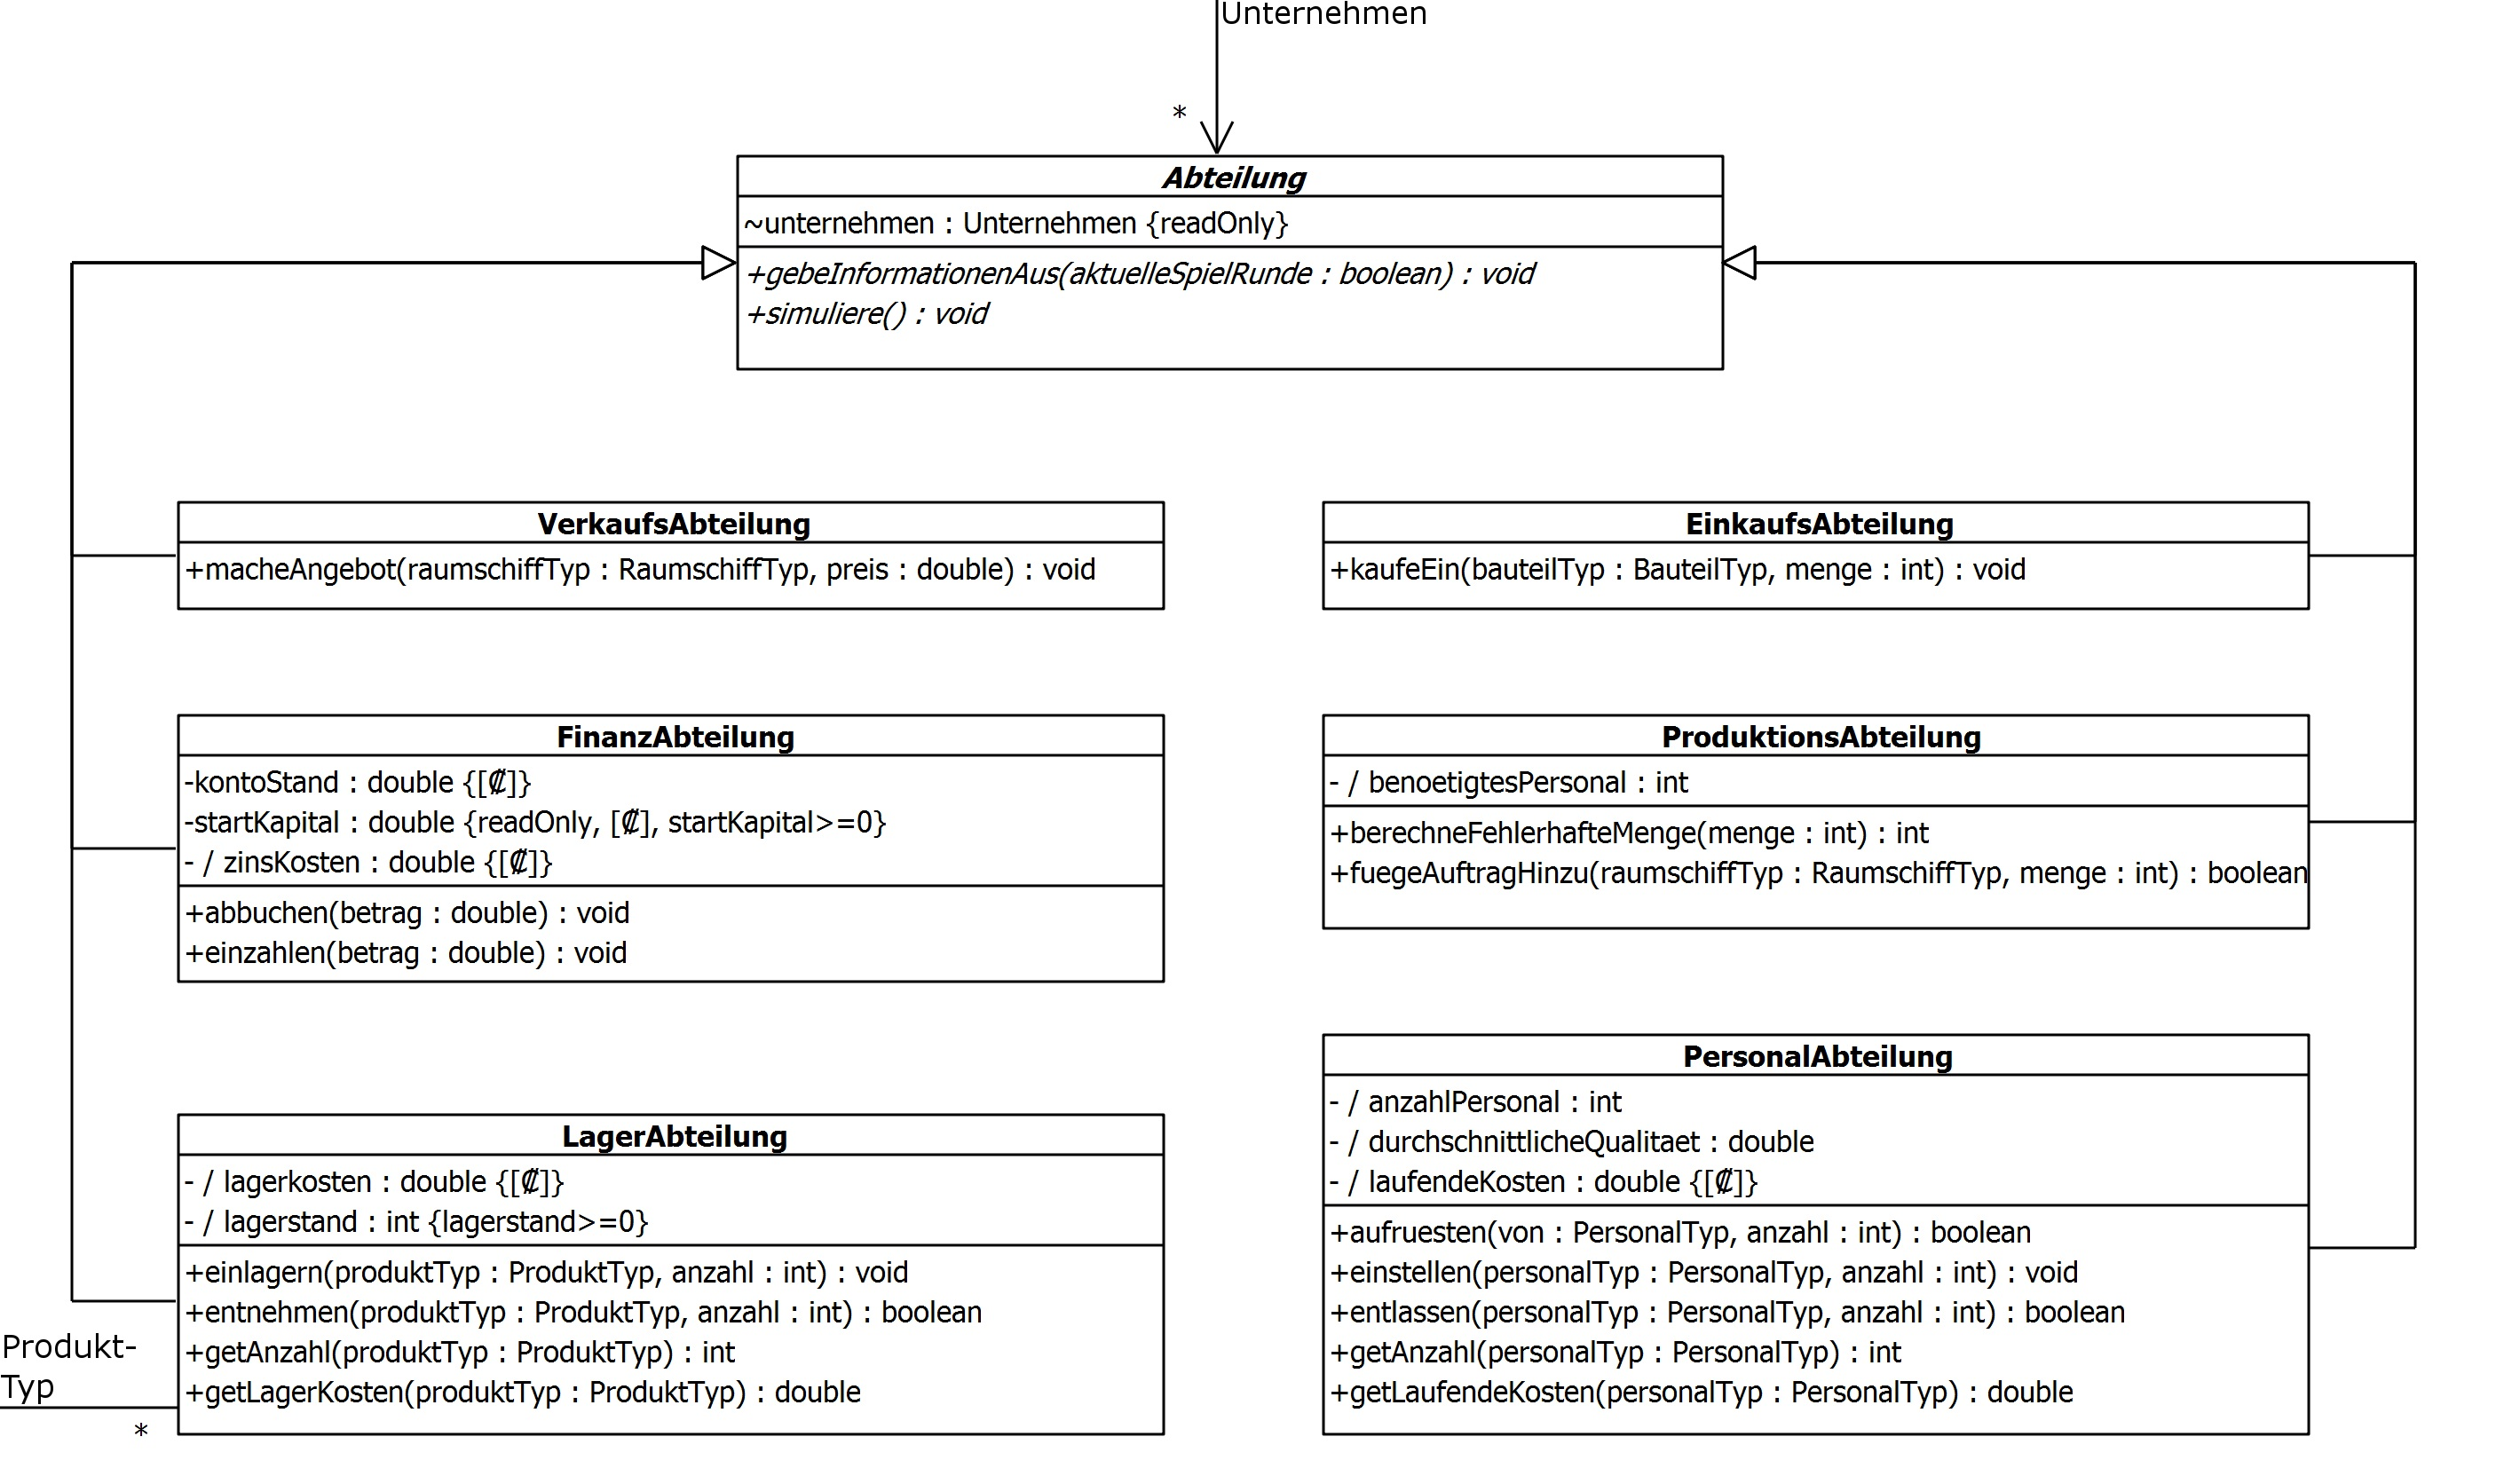
\includegraphics[width=\textwidth]{30_Fachkonzept/20_Entwurf/abteilung}
     \caption{Klassendiagramm - Abteilungen}
     \label{img:fachkonzept-entwurf-abteilung}
\end{figure}

Ein produzierendes Unternehmen besteht aus verschiedenen Abteilungen, zu denen klassischerweise der Einkauf, die Produktion und der Verkauf zählen. Für das Planspiel wurden drei zusätzliche Abteilungen eingeführt: Finanzen, Lager und Personal. Dies folgt nicht in allen Punkten der Realität, dient aber auf der Ebene der Modellierung der einheitlichen Verwaltung aller Teile des Unternehmens. Jede \textit{Abteilung} kann dabei durch \textit{gebeInformationenAus()} Informationen zu dem sie betreffenden Kontext ausgeben. Mit Hilfe des Parameters \textit{aktuelleSpielRunde} lässt sich steuern, ob sich die Informationen auf die aktuelle oder die zurückliegende Spielrunde beziehen sollen, was vor allem im Bereich des Verkaufs interessant ist.

\begin{seList}
\item \textbf{EinkaufsAbteilung:} Diese Abteilung dient lediglich dem Einkauf von Bauteilen.
\item \textbf{ProduktionsAbteilung:} Hier können Produktionsaufträge hinzugefügt werden, die im Laufe der SpielRunde abgearbeitet werden. Dabei muss ein Überblick über das noch zur Verfügung stehende Personal behalten werden. Bei der Simulation können zudem - abhängig von der Qualität des Personals - fehlerhafte Raumschiffe entstehen, die zusätzliche Kosten verursachen.
\item \textbf{VerkaufsAbteilung:} Hier können Verkaufsangebote gemacht werden, die sich immer auf einen bestimmten Raumschifftypen beziehen. Dabei wird am Ende der Runde versucht, so viele der dann vorhandenen Raumschiffe dieses Typs - Lagerbestände sowie frisch produzierte - zum angegebenen Preis abzusetzen.
\item \textbf{Finanzabteilung:} Das Unternehmen verwaltet hier seine Finanzen. Der Einfachheit halber beinhaltet dies die Abstraktion eines Kontos, das das Hauptgeschäftskonto des Unternehmens darstellt. Daher gibt es Methoden zum \textit{einzahlen()} und \textit{abbuchen()} von Geldbeträgen. Eine Unterdeckung des Kontso am Rundenende führt zu Zinskosten, die abhängig vom Zinssatz zur kurzfristigen Refinanzierung des Kapitalmarkts anfallen. Zur Berechnung des \textit{ROI} am Ende muss auch das zu Beginn vorhandene Startkapital festgehalten werden.
\item \textbf{PersonalAbteilung:} Diese verwaltet das angeworbene Personal, welches in verschiedenen Qualitätsstufen vorliegen kann. Die Gesamtanzahl des Personals beeinflusst dabei die Produktionskapazität, die durchschnittliche Qualität beeinflusst die Fehlerrate. Zusätzlich entstehen laufende Kosten, die bei der Simulation der Runde abgebucht werden. Spieler können Personal einstellen, aufrüsten oder je nach Situation auch entlassen.
\item \textbf{LagerAbteilung:} Bauteile und Raumschiffe müssen nicht sofort verbaut oder verkauft werden, sie werden zunächst in das Lager des Unternehmens gelegt. Daher besteht eine Beziehung zur Klasse \textit{ProduktTyp}, die ergänzt wird durch die assoziative Klasse \textit{Menge}. Abhängig vom Lagerstand, der die Summe der benötigten Lagerplatzeinheiten aller gelagerten Einheiten darstellt, entstehen zum Ende einer Runde Lagerkosten.
\end{seList}

\subsection{Die Transaktionen}
\begin{figure}[ht]
     \centering
     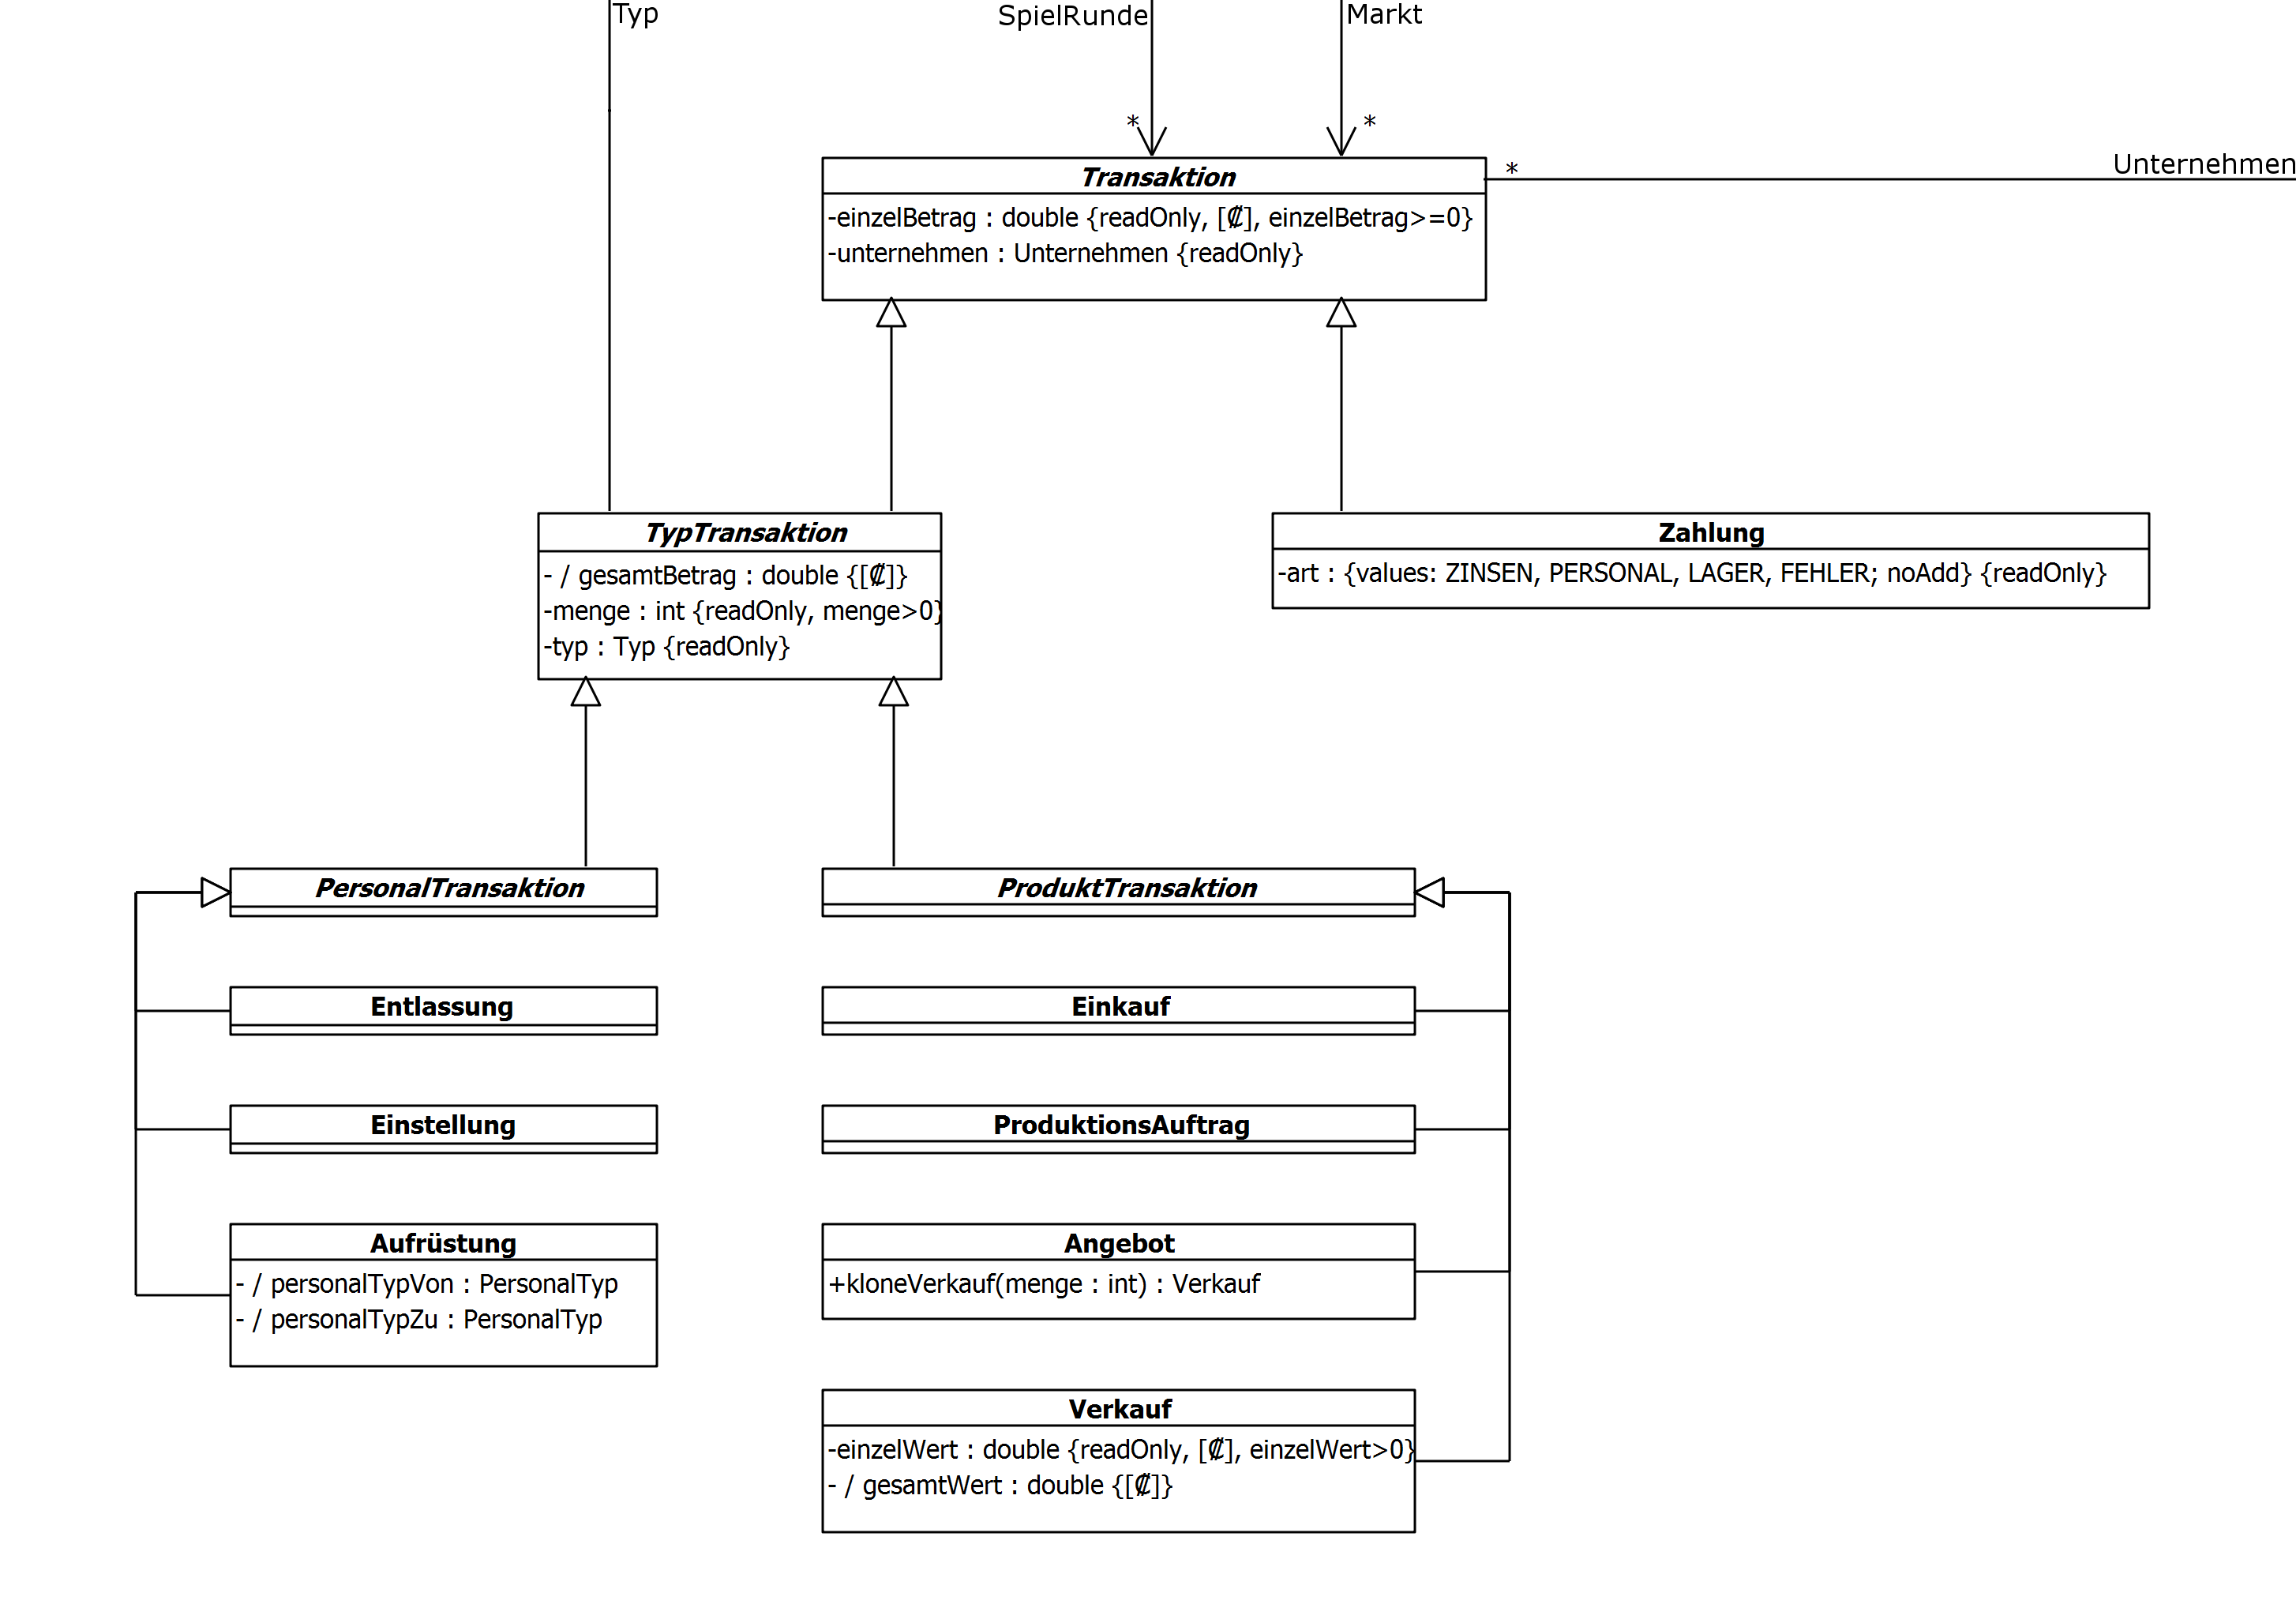
\includegraphics[width=\textwidth]{30_Fachkonzept/20_Entwurf/transaktion}
     \caption{Klassendiagramm - Abteilungen}
     \label{img:fachkonzept-entwurf-abteilung}
\end{figure}
Wie bereits erwähnt müssen Transaktionen, die Spieler durchführen, dauerhaft gespeichert werden, um so die Unternehmen abschließend bewerten zu können. Hierzu sind zwar nicht alle Transaktionen, die auch tatsächlich anfallen, relevant, allerdings scheint eine Speicherung aller einerseits konsequent und ermöglicht andererseits in Zukunft relativ einfach das Hinzufügen einer Funktionalität zum Zurücknehmen bzw. Rückgängigmachen von Entscheidungen, die noch keine weiteren Auswirkungen hatten. Transaktionen stehen dabei fest mit einem Unternehmen in Beziehung und sind gekennzeichnet (mit Ausnahme der Entlassung) durch einen Betrag. Anlehnend an die Struktur der Märkte kann man hier jedoch wieder unterscheiden zwischen solchen Transaktionen, die mit Typen in Verbindung stehen, den \textit{TypTransaktionen}, und der \textit{Zahlung}. Die Typtransaktionen untergliedern sich dabei noch weiter in die \textit{PersonalTransaktionen} und \textit{ProduktTransaktionen}. Stehen sie mit einem Typ in Zusammenhang, wird auch eine Menge gespeichert (die assoziative Klasse wird aufgrund der 1:* Beziehung nicht benötigt), wodurch sich auch ein Gesamtbetrag ergibt.

Es war dabei notwendig, einige weitere Unterklassen wie \textit{Verkauf} abzuleiten, da an einigen Stellen durch die Spezialisierung weitere Daten abgespeichert werden müssen. Hier erschien es dann konsequent, auch die anderen möglichen Transaktionen in eigene Unterklassen auszulagern, auch wenn sie keine weitere Funktionalität bieten, und die Oberklassen abstrakt zu gestalten.

Es werden hier nur solche Transaktionen aufgeführt, die einer weiteren Erkärung bedürfen:

\begin{seList}
\item \textbf{Angebot:} Da ein Angebot im Regelfall in einen fast identischen \textit{Verkauf} übergeführt werden kann, der sich lediglich in der Menge unterscheiden kann, stellt diese Klasse die Methode \textit{kloneVerkauf()} zur Verfügung.
\item \textbf{Verkauf:} Für einen Verkauf soll auch der derzeitige Wert des Raumschifftypen, gemessen an der Summe der Kosten für alle benötigten Bauteile, gespeichert werden. Dies dient der Berechnung des Marktanteils, der einerseits aufgrund der mangelnden Vergleichbarkeit nicht nur anhand von Stückzahlen berechnet werden kann, andererseits nicht am Umsatz gemessen werden soll, da dies Unternehmen mit hohen Preisen in der Bewertung zu sehr bevorteilt.
\end{seList}

\autorende{}